All the systematics and statistical uncertainties (nuisance parameters) are included in the 
likelihood function along with the parameter of interest (POI). The POI is the \brThb of this analysis.
For the sake of convenience, we will denote \brThb as \rm{BR} in this section. The impact of nuisance
parameters (NP) on the \rm{BR} indicates which NP plays dominant role in the limit computation. To
see the impact, each NP is individually varied by $\pm 1 \sigma$ of its pre-fit value and the 
corresponding change in the \rm{BR} is computed. The distribution of post-fit pulls and impacts of 
nuisance parameters is shown in Figures~\ref{fig:nuisImpact1},~\ref{fig:nuisImpact2},~\ref{fig:nuisImpact3}, and \ref{fig:nuisImpact4}, using $\mjj$ from exclusive event categories based on \PQc tagging 
for $\mHp = 120$ \GeV from \ljets channel. In these figures, $\theta_0$ is the pre-fit value, 
$\widehat{\theta}$ is the post-fit value, and $\Delta\theta = 1$ is the difference in the uncertainties 
from pre and post-fit values. The $\widehat{\rm{BR}}$ is the best-fit value of $\rm{BR}$. 
The $\Delta\widehat{\rm{BR}}$ is the change in the value of $\widehat{\rm{BR}}$ when the pull of a nuisance 
parameter is varied $\pm 1 \sigma$ of its pre-fit value. 

Larger the value of $\Delta\widehat{\rm{BR}}$, larger is the correlation between $\rm{BR}$ and the 
corresponding nuisance parameter. Also, if the change in \rm{BR} is positive (negative) when 
an NP is varied $+1\sigma$ ($-1\sigma$) of its pre-fit value then they are positively correlated. 
However, if the change in \rm{BR} is 
opposite to the variation in NP then they are said to be anti-correlated. One of the most important
feature of the plots shown in Figures~\ref{fig:nuisImpact1},~\ref{fig:nuisImpact2},~\ref{fig:nuisImpact3}, and \ref{fig:nuisImpact4} is the ordering (or indexing) of the NPs. The nuisance parameter having
highest impact on the \rm{BR} is placed at the top (index is 1) of the plot. Those placed at bottom
have relatively small impact on \rm{BR} thereby don't affect the limit. One another important feature
in these plots is the $\pm 1\sigma$ values of the NPs. If an NP hase smaller $\pm 1\sigma$ value then
it is said to be constrained. In such case the constraint on that NP has to be relieved by scrutinizing
its pre-fit values. A large constraint on the NPs leads to larger mismatch between the expected and
observed limits. The acronym used in these plots for statistical uncertainties are given in 
Table~\ref{tab:autoMCStat} for reference. 
 
\begin{table}
\caption{Acronym used in the impact plots for naming statistical nuisance parameters.} 
\label{tab:autoMCStat}
\begin{center}
\begin{tabular}{ccc}
\hline
\hline
{\bf{Acronym}} & {\bf{channel}} & {\bf{Event category}}\\
\hline
\hline
binch1    & \mujets & exclusive loose\\
binch2    & \mujets & exclusive medium\\
binch3    & \mujets & exclusive tight\\
binch4    & \ejets  & exclusive loose\\
binch5    & \ejets  & exclusive medium\\
binch6    & \ejets  & exclusive tight\\
\hline
\end{tabular}
\end{center}
\end{table} 
 
\begin{figure}
\begin{center}
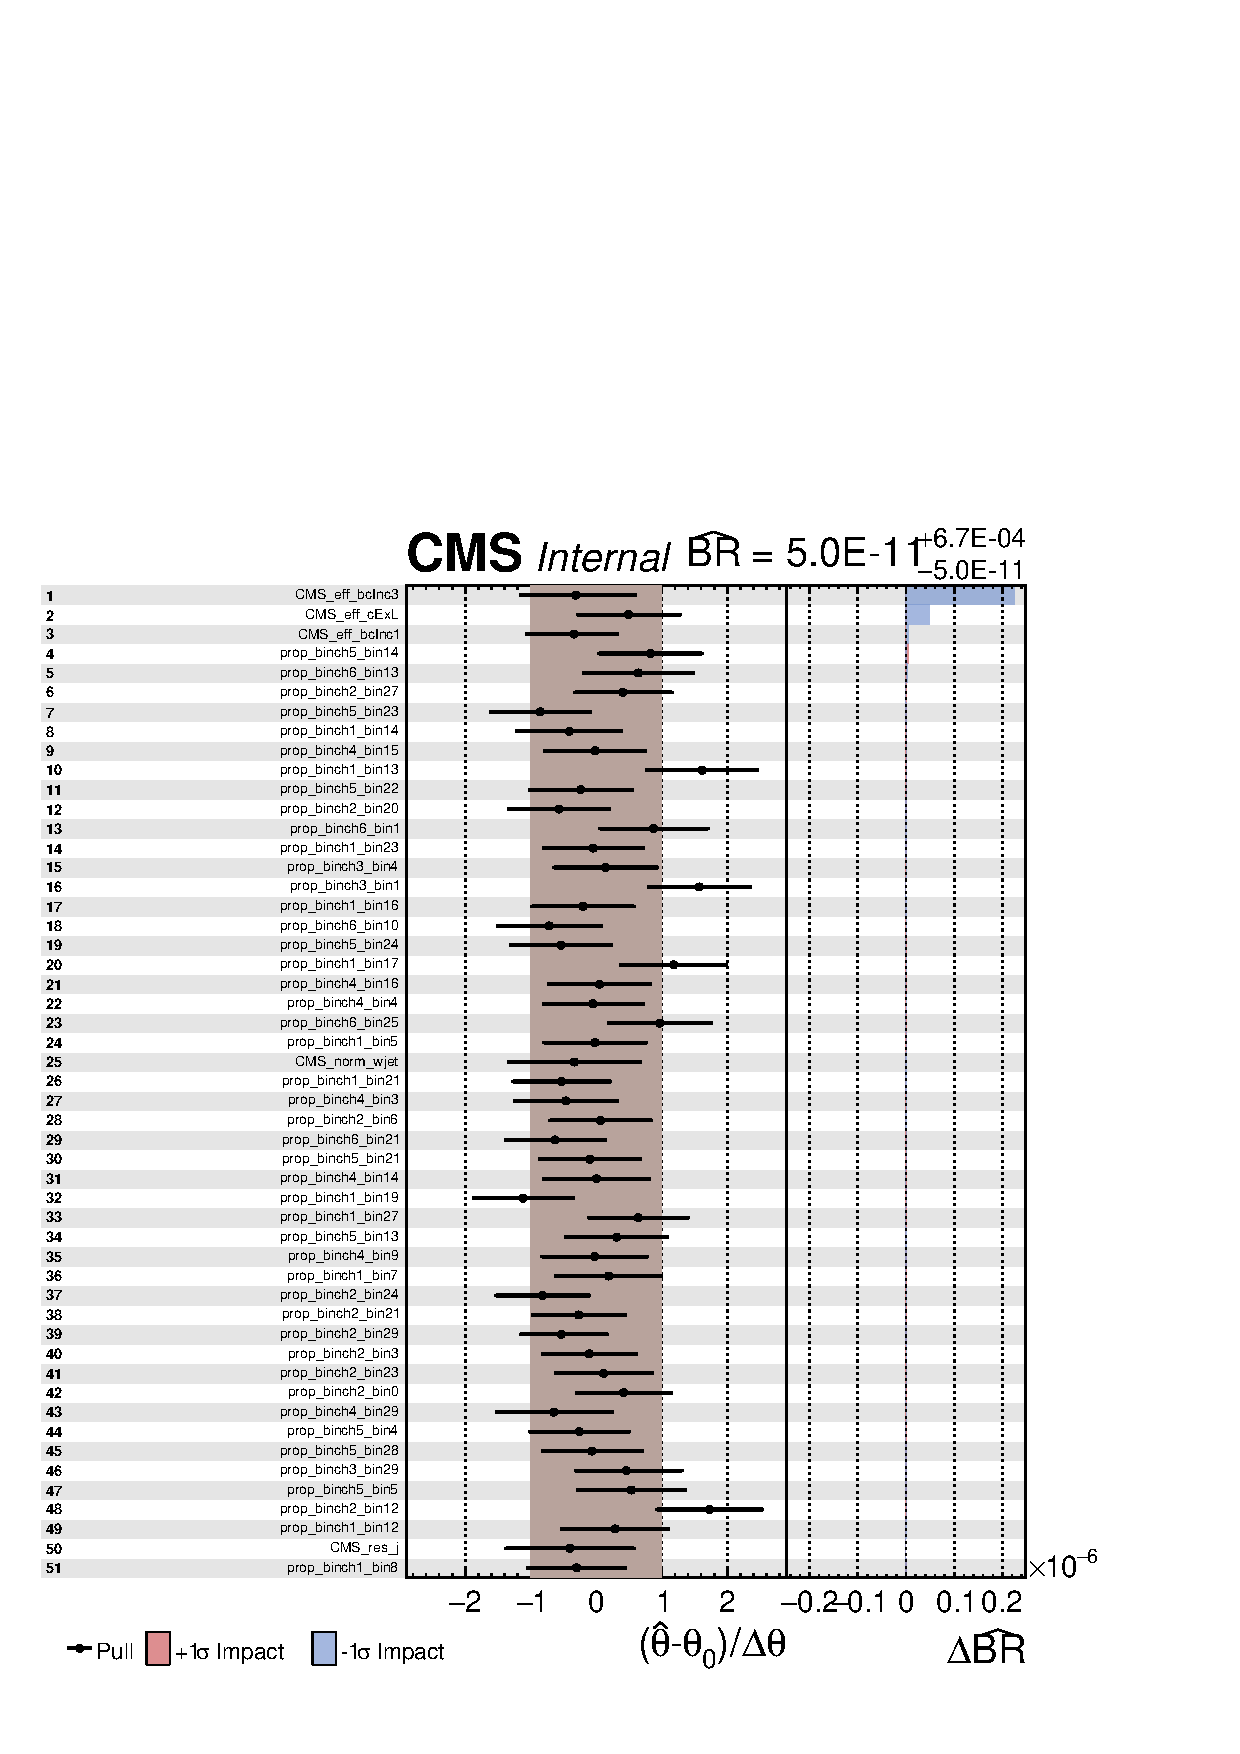
\includegraphics[width=1.0\textwidth]{Image/MLFit/ImpactNuis/nuisImpact1.pdf}
 \caption{Distribution of post-fit pulls and impacts of nuisance parameters from
     exclusive event categories based on charm-tagging for $\mHp=120$
     \GeV from \ljets channel. Contd ...}
\label{fig:nuisImpact1}
\end{center}
\end{figure}

\begin{figure}
\begin{center}
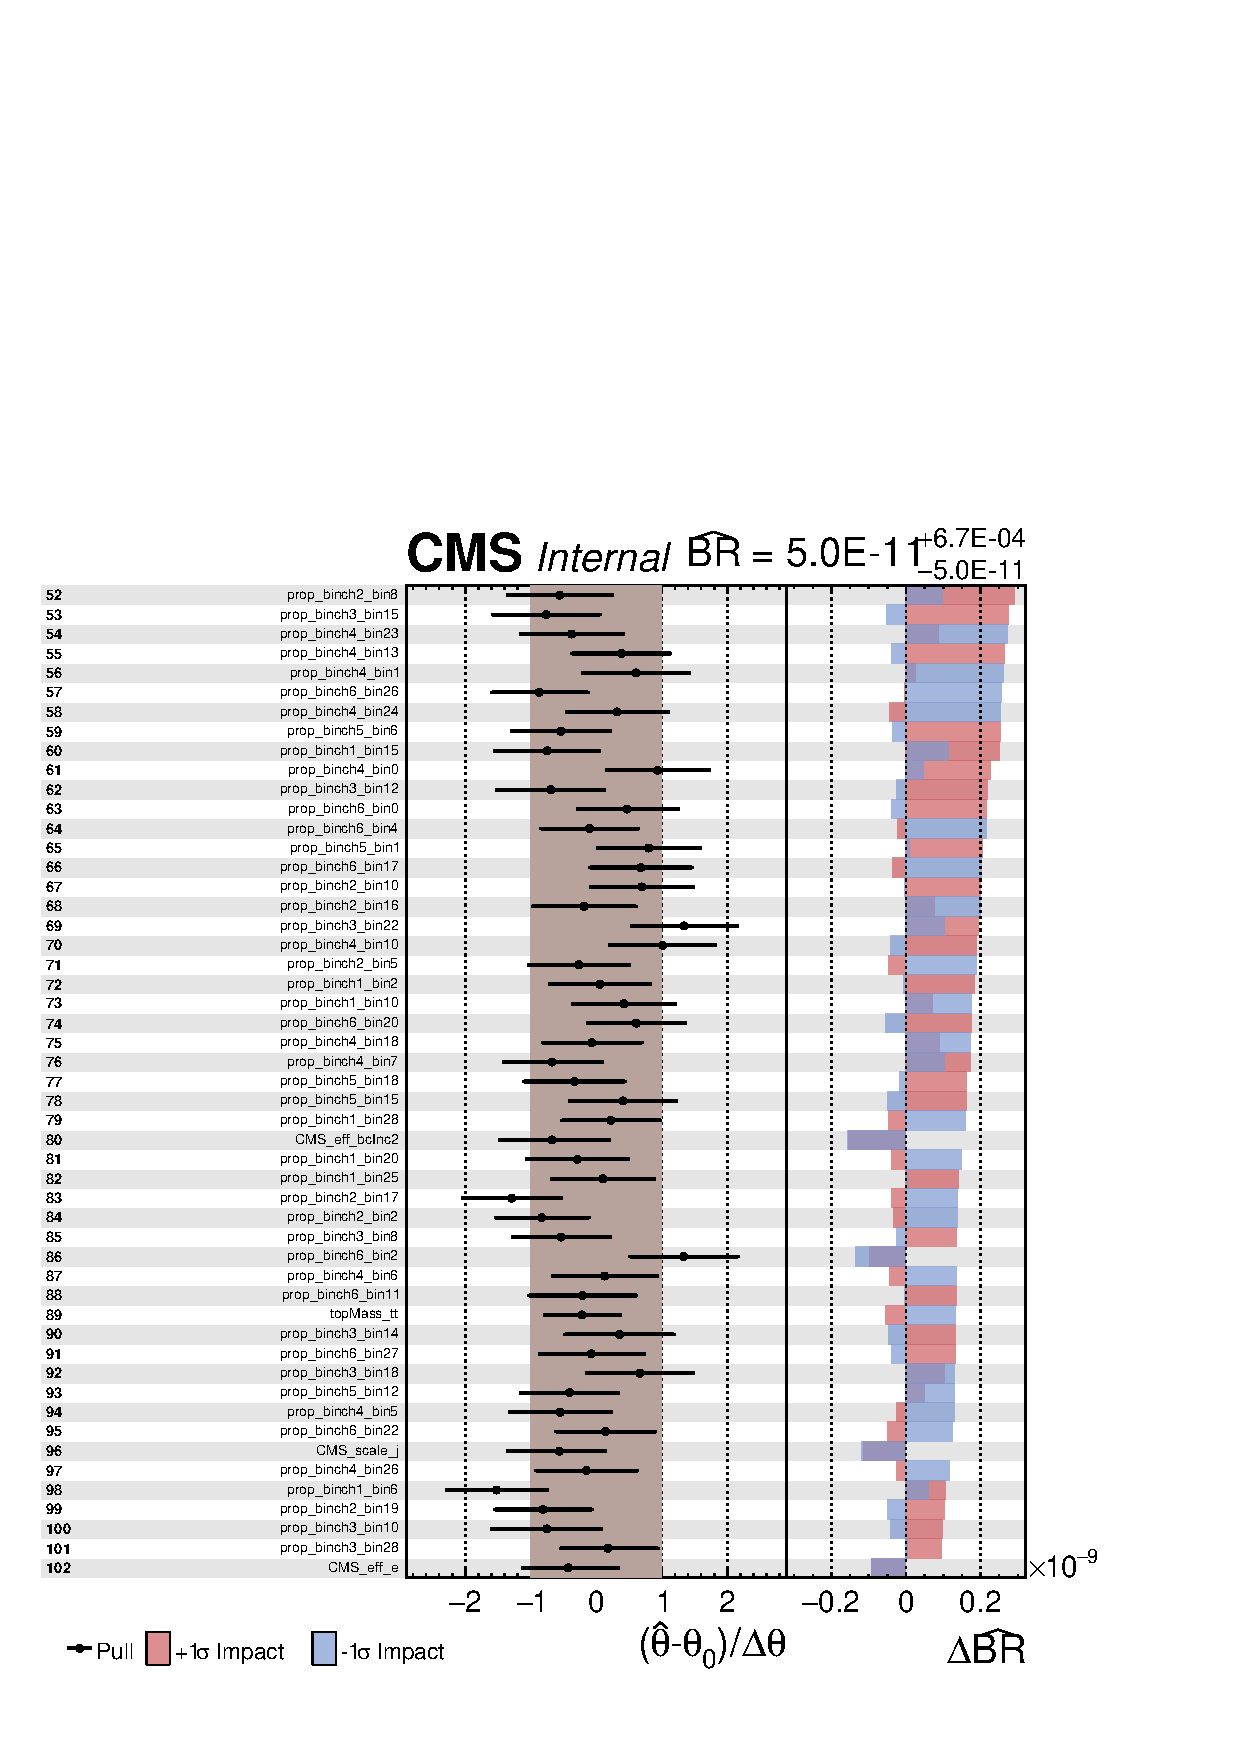
\includegraphics[width=1.0\textwidth]{Image/MLFit/ImpactNuis/nuisImpact2.pdf}
 \caption{Distribution of post-fit pulls and impacts of nuisance parameters from
     exclusive event categories based on charm-tagging for $\mHp=120$
     \GeV from \ljets channel. Contd ...}
\label{fig:nuisImpact2}
\end{center}
\end{figure}

\begin{figure}
\begin{center}
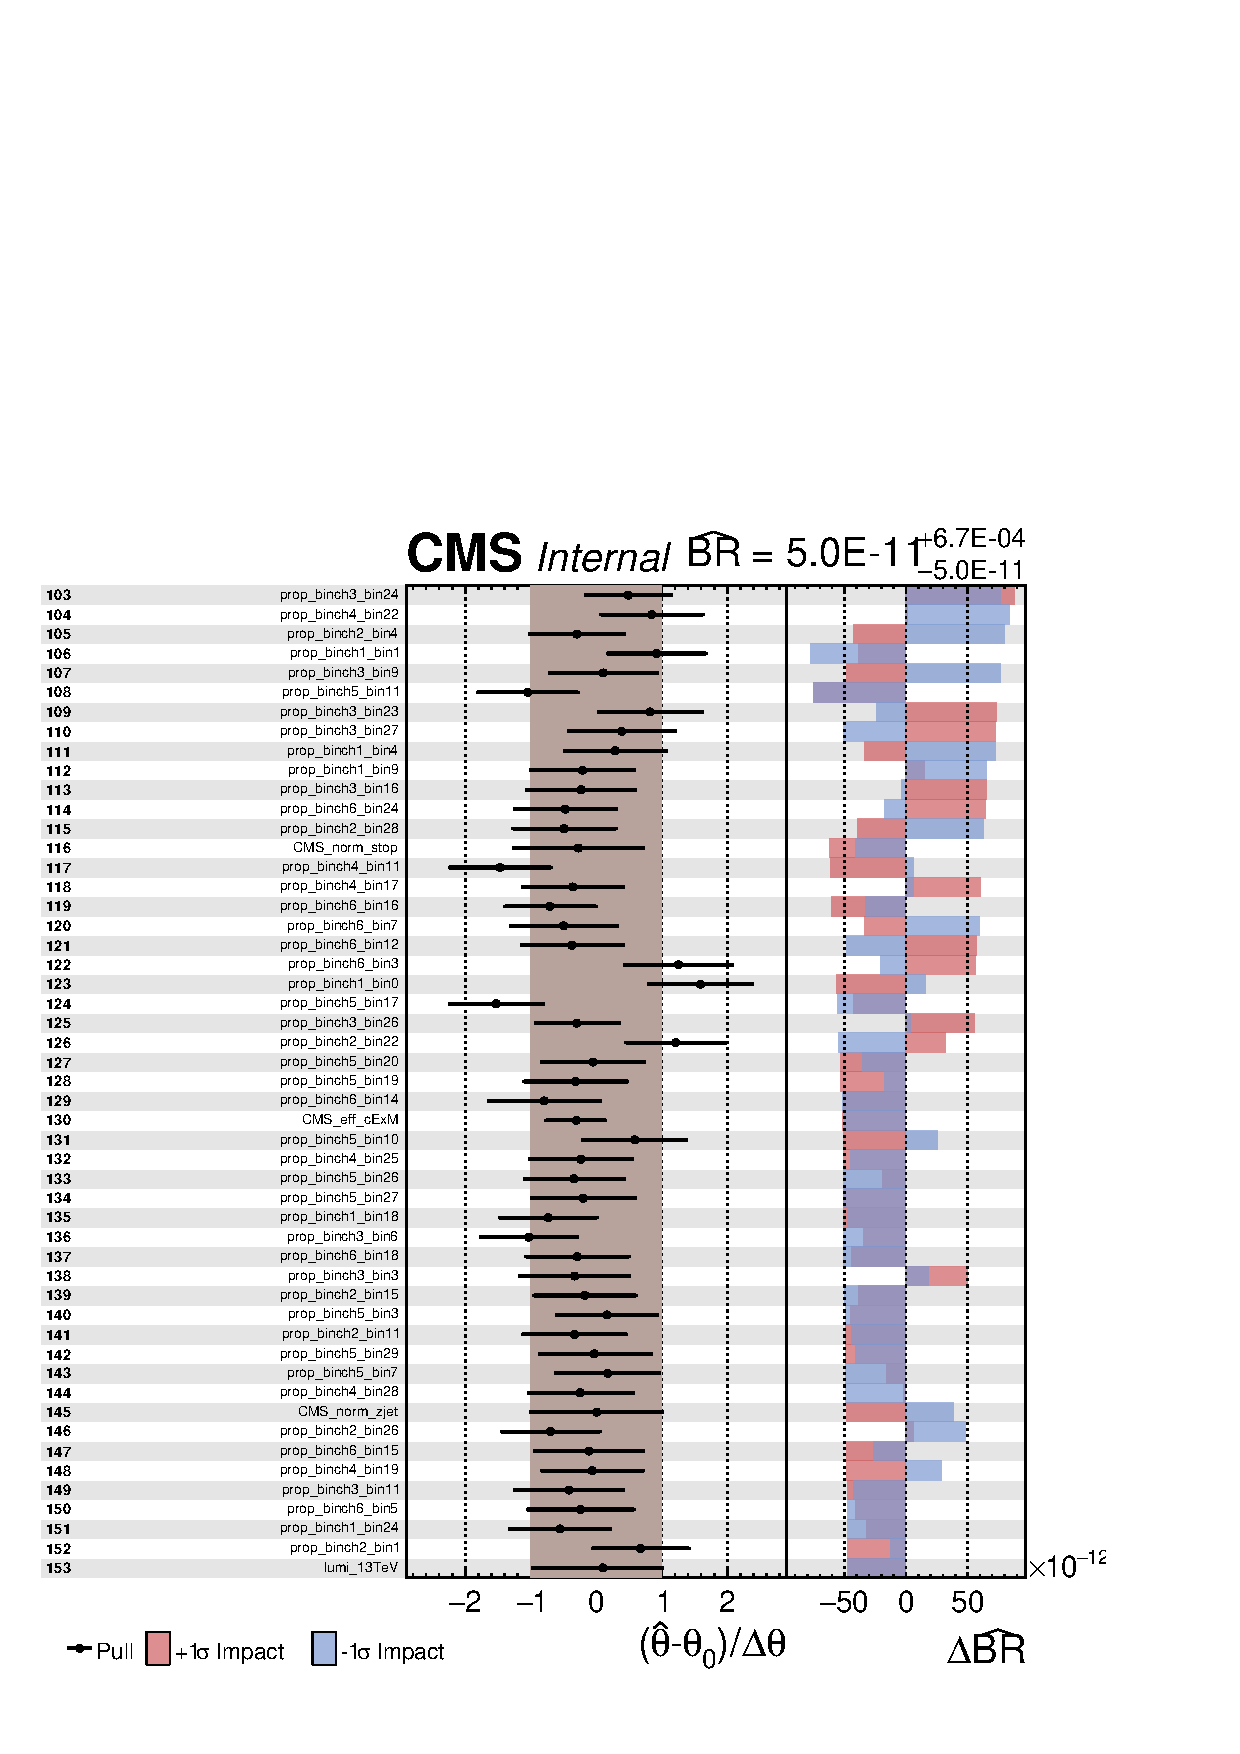
\includegraphics[width=1.0\textwidth]{Image/MLFit/ImpactNuis/nuisImpact3.pdf}
 \caption{Distribution of post-fit pulls and impacts of nuisance parameters from
     exclusive event categories based on charm-tagging for $\mHp=120$
     \GeV from \ljets channel. Contd ...}
\label{fig:nuisImpact3}
\end{center}
\end{figure}

\begin{figure}
\begin{center}
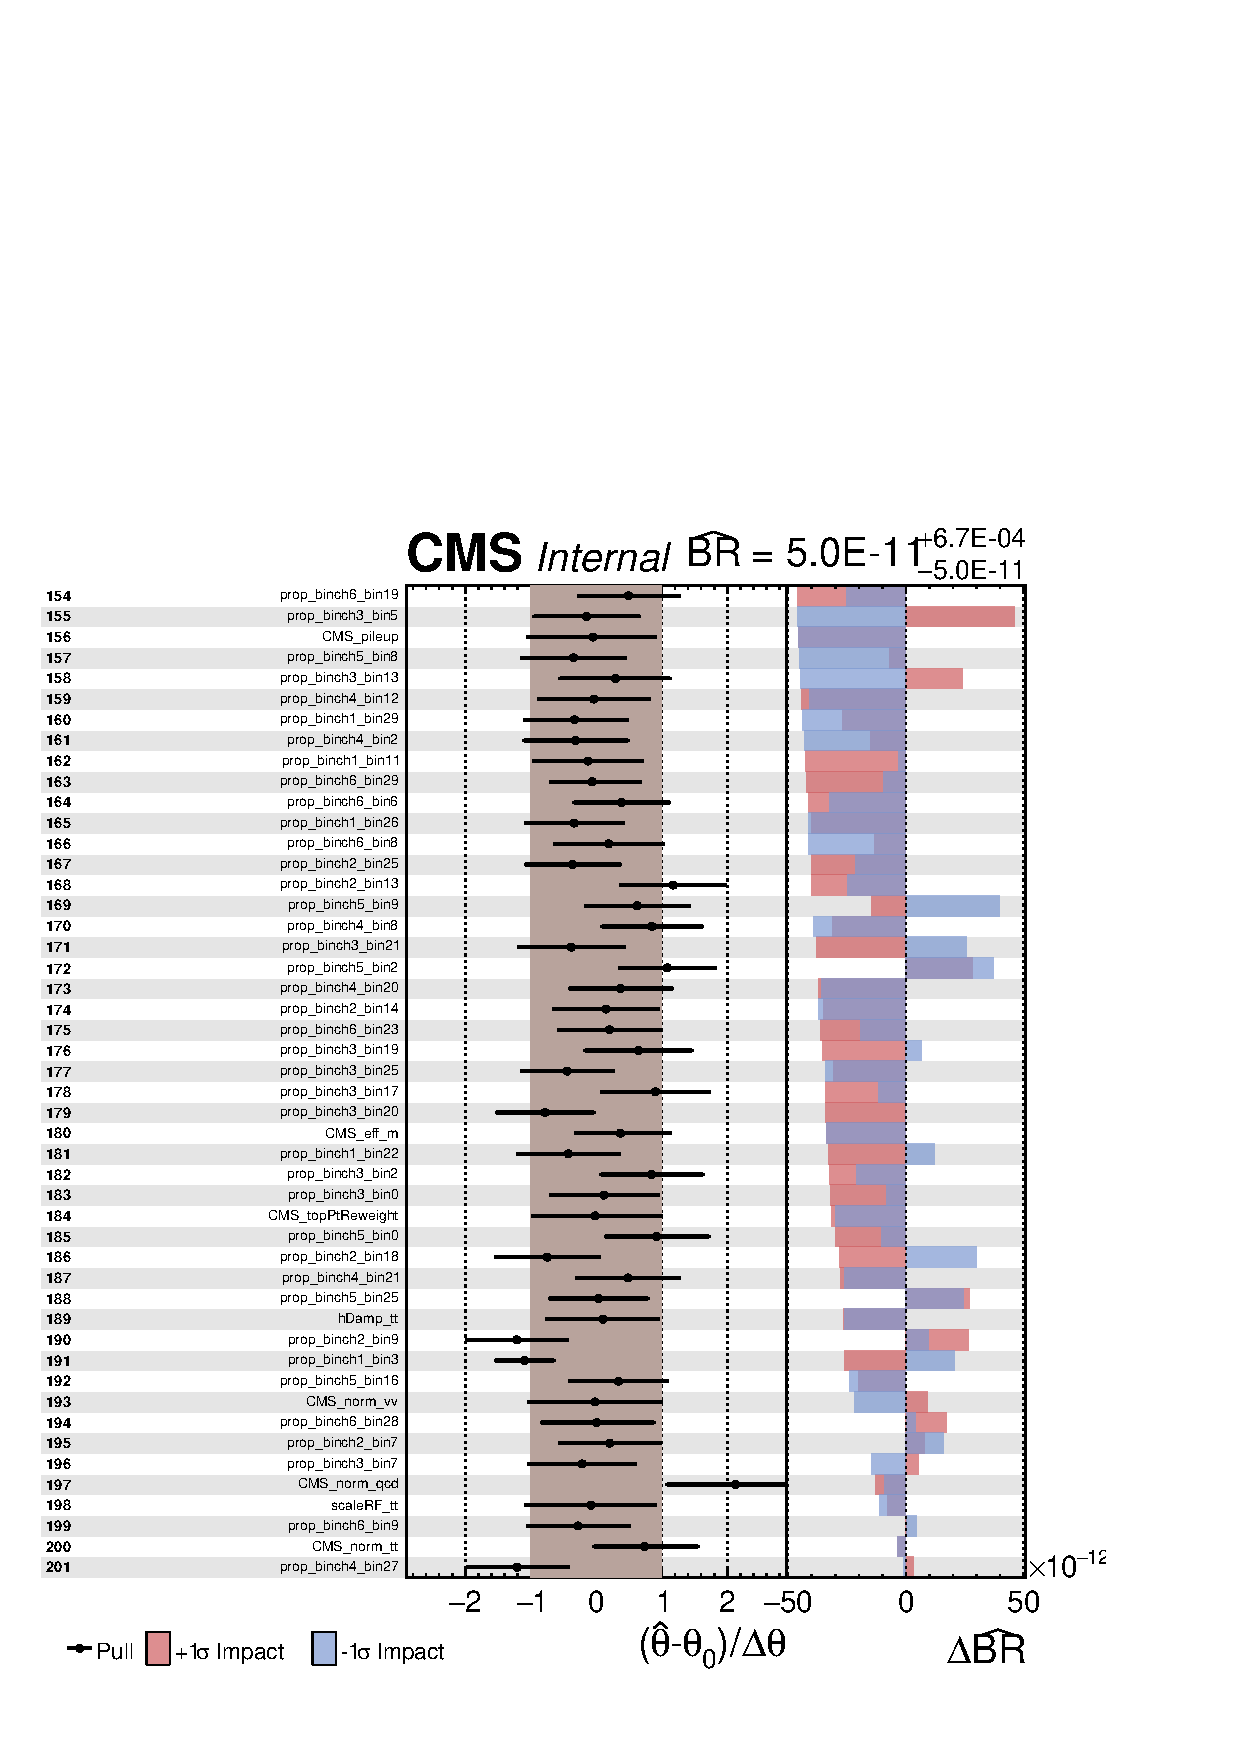
\includegraphics[width=1.0\textwidth]{Image/MLFit/ImpactNuis/nuisImpact4.pdf}
 \caption{Distribution of post-fit pulls and impacts of nuisance parameters from
     exclusive event categories based on charm-tagging for $\mHp=120$
     \GeV from \ljets channel.}
\label{fig:nuisImpact4}
\end{center}
\end{figure}

